\documentclass[tikz,border=8pt]{standalone}
% Shared look for every TikZ diagram. Load with \input{../../tools/tikz-style.tex}
\usepackage[T1]{fontenc}
\usepackage{lmodern}
\renewcommand{\sfdefault}{lmr}  % diagrams use the same serif as the text
\usetikzlibrary{arrows.meta, positioning, shapes.geometric, calc, fit, backgrounds}
\definecolor{cblue}{HTML}{4C78A8}
\definecolor{corange}{HTML}{F58518}
\definecolor{cgreen}{HTML}{54A24B}
\definecolor{cred}{HTML}{E45756}
\definecolor{cpurple}{HTML}{B279A2}
\definecolor{cgrey}{HTML}{6B6B6B}
\tikzset{
  every picture/.style={font=\sffamily, line width=1.2pt},
  box/.style={draw=#1, fill=#1!12, rounded corners=4pt, align=center, inner sep=7pt, minimum height=1.1cm},
  box/.default=cgrey,
  arrow/.style={-{Stealth[length=3mm]}, draw=cgrey, line width=1.4pt},
  title/.style={font=\sffamily\bfseries\Large},
  note/.style={font=\sffamily\small, text=cgrey, align=center},
}
\AtBeginDocument{\hyphenpenalty=10000 \exhyphenpenalty=10000}

\begin{document}
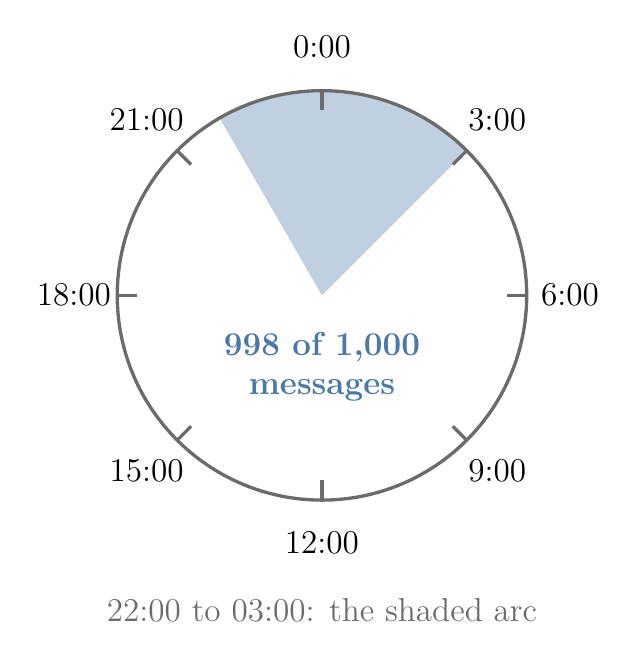
\begin{tikzpicture}[every node/.append style={font=\sffamily\large}]
\tikzset{note/.style={font=\sffamily\large, text=cgrey, align=center}}
  \def\R{2.6}
  % shaded night arc 22:00 -> 03:00 (clock angle: 90 - 15*h)
  \fill[cblue!35] (0,0) -- (90-15*22:\R) arc[start angle=90-15*22, end angle=90-15*27, radius=\R] -- cycle;
  \draw[cgrey] (0,0) circle (\R);
  \foreach \h in {0,3,...,21} {
    \draw[cgrey] (90-15*\h:\R) -- (90-15*\h:\R-0.25);
    \node[font=\sffamily\large] at (90-15*\h:\R+0.55) {\h:00};
  }
  \node[font=\sffamily\bfseries\large, text=cblue, align=center] at (0,-0.9) {998 of 1,000\\messages};
  \node[note] at (0,-4.0) {22:00 to 03:00: the shaded arc};
\end{tikzpicture}
\end{document}
